%
% GNU courseware, XIN YUAN, 2018
%

\section{团队协作}

\frame{
\centerline{\textbf{\Huge{团队协作}}}
}

\frame{\frametitle{角色分工}
\begin{table}[htbp]
\centering
\begin{tabular}{|p{0.3\textwidth}<{\centering}|p{0.6\textwidth}|}
\hline
\textbf{角色} & \textbf{分工}\\
\hline
\rowcolor[rgb]{0.0, 0.8, 0.8}
项目经理 & 产品设计和工程监督\\
\hline
架构师 & 软件架构设计\\
\hline
\rowcolor[rgb]{0.0, 0.8, 0.8}
程序员 & 程序开发\\
\hline
测试员 & 软件测试\\
\hline
\end{tabular}
\end{table}
}

\frame{\frametitle{工具链}
\begin{table}[htbp]
\centering
\begin{tabular}{|p{0.3\textwidth}<{\centering}|p{0.6\textwidth}|}
\hline
\textbf{名称} & \textbf{工具}\\
\hline
\rowcolor[rgb]{0.0, 0.8, 0.8}
版本控制 & Git, fossil\\
\hline
持续集成 & Jenkins, Appveyor\\
\hline
\rowcolor[rgb]{0.0, 0.8, 0.8}
构建工具 & CMake, QMake\\
\hline
规范检查 & cpplint\\
\hline
\rowcolor[rgb]{0.0, 0.8, 0.8}
静态分析 & cppcheck\\
\hline
复杂度分析 & cppncss\\
\hline
\rowcolor[rgb]{0.0, 0.8, 0.8}
单元测试覆盖率 & OpenCppCoverage, gcov\\
\hline
\end{tabular}
\end{table}
}

\frame{\frametitle{工作流程}
单人工作和多人协作是不同的。

~

\begin{itemize}
\item<1-> 瀑布流程:需求-分析-概要设计-详细设计-编码实现-测试-发布-反馈
\item<2-> 敏捷流程:用户故事-场景-测试用例-迭代-反馈
\end{itemize}
}

\frame{\frametitle{工作流程}
\begin{minipage}[t]{\textwidth}
git flow:
\end{minipage}

~

\uncover<2->{
\noindent
\begin{minipage}[b]{\textwidth}
\begin{figure}[hb]
\centering
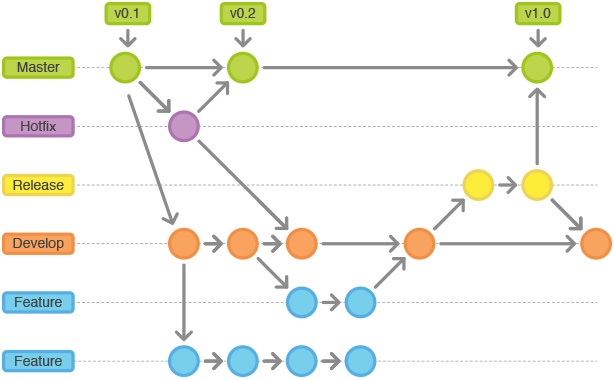
\includegraphics[width=0.8\textwidth]{topics/team-files/wf-git.png}
\end{figure}
\end{minipage}
}
}

\frame{\frametitle{工作流程}
\begin{minipage}[t]{\textwidth}
github flow:
\end{minipage}

~

\uncover<2->{
\noindent
\begin{minipage}[b]{\textwidth}
\begin{figure}[hb]
\centering
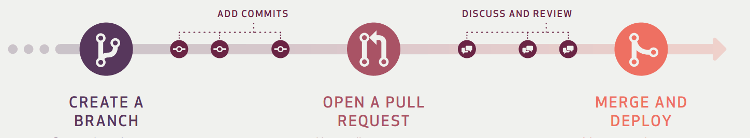
\includegraphics[width=0.8\textwidth]{topics/team-files/wf-github.png}
\end{figure}
\end{minipage}
}
}

\frame{\frametitle{GitHub工作流程}
\begin{figure}[hb]
\centering
\animategraphics[height=1.5in, autoplay, controls]{1}{topics/team-files/wf-github-a}{1}{6}
\end{figure}
}

\frame{\frametitle{工作流程}
\begin{minipage}[t]{\textwidth}
GitLab工作流程分为持续发布和版本发布:
\end{minipage}

~

\begin{minipage}[b]{\textwidth}
\noindent
\begin{figure}[hb]
\centering
\uncover<2->{
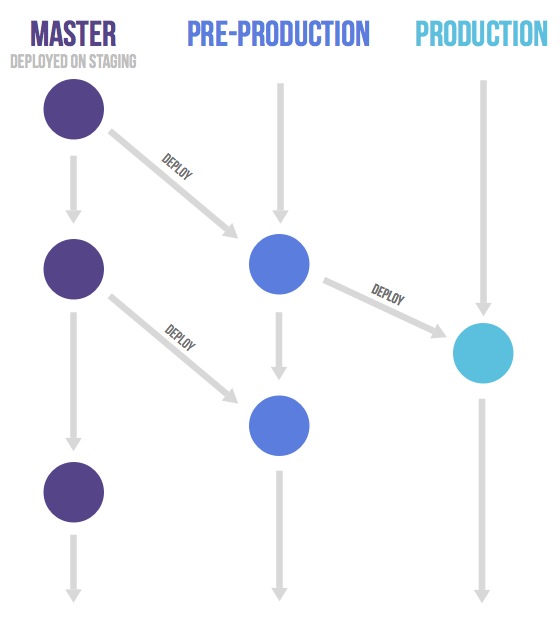
\includegraphics[width=0.4\textwidth]{topics/team-files/wf-gitlab1.png}
}
~
\uncover<3->{
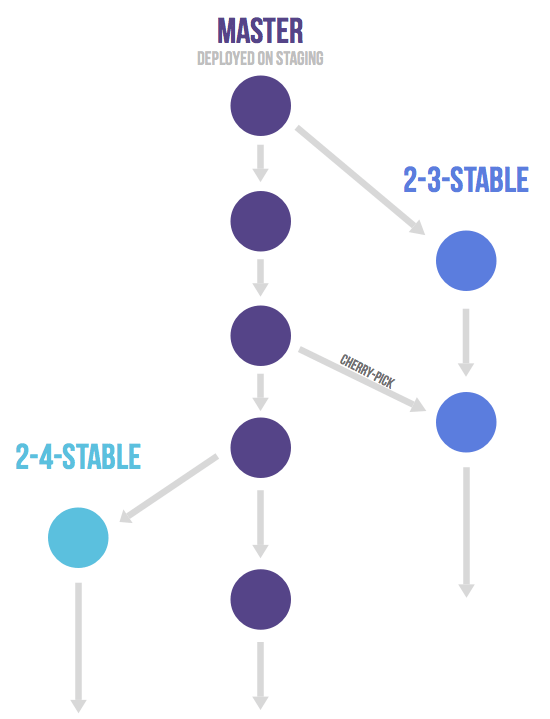
\includegraphics[width=0.4\textwidth]{topics/team-files/wf-gitlab2.png}
}
\end{figure}
\end{minipage}
}

\frame{\frametitle{工作流程}
\begin{minipage}[t]{\textwidth}
fossil flow:
\end{minipage}

~

\uncover<2->{
\noindent
\begin{minipage}[b]{\textwidth}
\begin{figure}[hb]
\centering
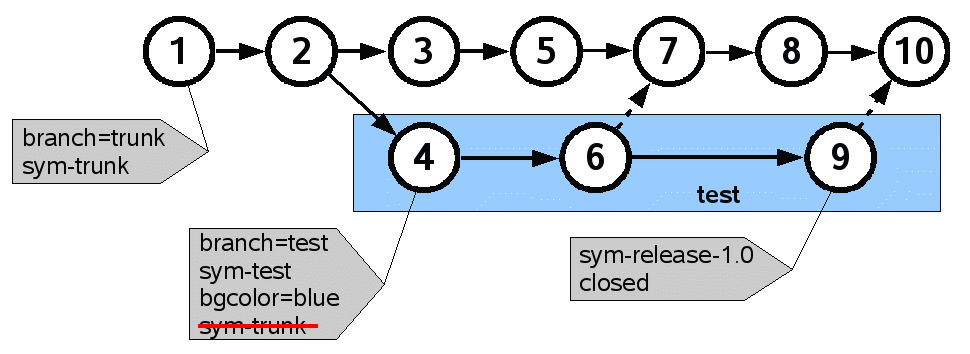
\includegraphics[width=0.8\textwidth]{topics/team-files/wf-fossil.png}
\end{figure}
\end{minipage}
}
}

\frame{\frametitle{工作流程}

一般地,某一个人做一个或多个功能或者修订一个或多个issue/ticket就要开一个新的分支,
完成后关闭或删除。
}

\frame{\frametitle{文档}
\begin{table}[htbp]
\centering
\begin{tabular}{|p{0.6\textwidth}|p{0.3\textwidth}|}
\hline
\textbf{内容} & \textbf{格式}\\
\hline
\rowcolor[rgb]{0.0, 0.9, 0.8}
需求分析 & Markdown(可以在线协作)\\
\hline
技术分析 & Markdown(可以在线协作)\\
\hline
\rowcolor[rgb]{0.0, 0.9, 0.8}
规划分析(思维导图,规划系统和行动全景图) & Markdown\\
\hline
测试计划 & Markdown(可以在线协作)\\
\hline
\rowcolor[rgb]{0.0, 0.9, 0.8}
甘特图/燃尽图 & LaTex\\
\hline
用例图 & LaTex \\
\hline
\rowcolor[rgb]{0.0, 0.9, 0.8}
类图 & LaTex\\
\hline
顺序协作图 & LaTex\\
\hline
\end{tabular}
\end{table}
}

%end
